\documentclass{article}
% chktex-file 44
% chktex-file 8
% chktex-file 18
% chktex-file 35
\usepackage[margin=1in]{geometry}
\usepackage{amsmath}
\usepackage{amssymb}
\usepackage{bm}
\usepackage{pdfpages}
\usepackage{graphicx}
\usepackage{mathtools}
\usepackage{eurosym}
\usepackage[hidelinks]{hyperref}
\usepackage{float}

\usepackage{fancyhdr}
\pagestyle{fancy}
\lhead{Ahou L. -  Ahou S. - Fiorini L. - Portier A.} % controls the left corner of the header
\chead{} % controls the center of the header
\rhead{Groupe 49} % controls the right corner of the header
\lfoot{} % controls the left corner of the footer
\cfoot{} % controls the center of the footer
\cfoot{~\thepage} % controls the right corner of the footer
\usepackage{titlesec}

% Commands for physic unit
\newcommand{\unit}[1]{[\mathrm{#1}]}

\begin{document}

\section*{Question 4A}
Puisque nous nous intéressons seulement aux bilans de productions/consommations et du niveau du bassin
sur des périodes de $T \unit{h}$, nous pouvons exprimer toutes nos variables en fonction de cette période.\\
Voici deux tableaux reprenant les notations principales utilisées dans cette seconde partie \footnote{Toutes autres notations utilisées dans la suite seront définies lorsque celles-ci seront introduites} : 

\begin{table}[h!]
    \centering
    \renewcommand{\arraystretch}{1.5}% Add spacing between rows : default value is 1
    \begin{tabular}{|c || c |} 
        \hline
        Nom & Signification\\
        \hline\hline
        $c_i$ & Capacité éolienne installée sur le i\textsuperscript{ème} site\\
        $t_j$ & Puissance à envoyer en turbinage choisie durant la j\textsuperscript{ème} période\\
        $p_j$ & Puissance de pompage choisie durant la j\textsuperscript{ème} période\\
        \hline
    \end{tabular}
    \caption{Table des notations des variables de décisions utilisées pour le modèle de la question 4.}
    \label{table:notations_variables_4}
\end{table}

\begin{table}[h!]
    \centering
    \renewcommand{\arraystretch}{1.5}% Add spacing between rows : default value is 1
    \begin{tabular}{|c || p{14cm} |} 
        \hline
        Nom & Signification\\
        \hline\hline
        $n$ & Nombre de sites éoliens \\
        $m$ & Nombre de périodes de $T \unit{h}$ dans une année\\
        $e_i(j)$ & Rendement éolien du i\textsuperscript{ème} site durant la j\textsuperscript{ème} période\\
        $a_j$ & Apport fluvial durant la j\textsuperscript{ème} période\\
        $\mathrm{cons}_j$ & Consommation énergétique durant la j\textsuperscript{ème} période\\
        $t_\mathrm{max}$ & Capacité maximale d'énergie générée par le turbinage (Sur une période de T heures)\\
        $p_\mathrm{max}$ & Capacité maximale de pompage (Sur une période de T heures)\\
        $\mathrm{stock}_\mathrm{max}$ & Capacité de stockage maximale\\
        $\eta$ & Rendement de turbinage\\
        $\mathrm{costs}$ & Vecteur donnant les valeurs du coût d'installation d'un site éolien  (onshore/offshore) \newline $\mathrm{costs}_i = $ Coût d'installation d'un site onshore si le site d'index $i$ est onshore, et inversement.\\  
        \hline
    \end{tabular}
    \caption{Table des notations des constantes utilisées pour le modèle.}
    \label{table:notations_constantes}
\end{table}

\noindent
Le modèle peut alors s'écrire ainsi :
\begin{align}
    \min_{c_{i},t_j,p_j} \quad &\mathrm{costs}^\intercal\mathbf{c} \nonumber\\
    \textrm{tel que} \quad & \sum_{i=0}^{n-1} c_i e_i(j) + \eta \cdot t_j - p_j \ge \mathrm{cons}_j \quad \forall j \in  \{ 0, \ldots, m-1 \}\label{eq:4A_contr1}\\
    & 0 \le \frac{\mathrm{stock}_\mathrm{max}}{2}  + \sum_{j=0}^{k} p_j - t_j + a_j \le  \mathrm{stock}_\mathrm{max} \quad \forall k \in \{ 0, \ldots, m-2 \}\label{eq:4A_contr2}\\
    & \sum_{j=0}^{m-1} p_j - t_j + a_j = 0 \label{eq:4A_contr3}\\
    & 0 \le c_i \le c_i^\mathrm{max} \quad \forall i \in  \{ 0, \ldots, n-1 \}  \label{eq:4A_contr4}\\
    & 0 \le \eta \cdot t_j \le  t_\mathrm{max} \quad \forall j \in  \{ 0, \ldots, m-1 \}  \label{eq:4A_contr5}\\
    & 0 \le p_j \le  p_\mathrm{max} \quad \forall j \in  \{ 0, \ldots, m-1 \} \label{eq:4A_contr6}
\end{align}

\newpage

La fonction objectif représente le coût total d'installation des éoliennes (en tenant compte des différences entre les installations \textit{offshore} et \textit{onshore}). \\
La contrainte \eqref{eq:4A_contr2} fait le bilan lié aux variations des opérations de turbinage/pompage décidées et de l'apport fluvial naturel depuis la période $t = 0$ jusqu'en toute période $t = k$ afin de calculer l'augmentation/la diminution du niveau de l'eau dans le bassin 
et imposer que le niveau de l'eau reste dans les limites du stockage maximal.\\
La contrainte \eqref{eq:4A_contr3} indique que le niveau final du bassin doit revenir au même niveau qu'initialement. Autrement dit, les opérations de turbinage/pompage et 
l'apport fluvial doivent se sommer à 0 à la fin de la dernière période.\\
Les contraintes \eqref{eq:4A_contr4}, \eqref{eq:4A_contr5} et \eqref{eq:4A_contr6} indiquent respectivement les bornes sur les capacités éoliennes maximales installables sur chaque site, 
les capacités maximales de turbinages et les capacités maximales de pompages pour des périodes de $T \unit{h}$, regroupées au niveau européen, bien entendu.
Nous avons cependant supposé pour la \eqref{eq:4A_contr5} contrainte, liée au turbinage, que la valeur $t_j$ est ce que 
nous extrayons du bassin, puis
la capacité $t_\mathrm{max}$ restreint alors l'énergie en sorte de la turbine($\eta \cdot t_j$), qui sert à la 
production électrique dans la condition \eqref{eq:4A_contr1}.

\newpage % Car il faudra rendre sur Gradescope en séparant les questions

\section*{Question 4B}
Suite à l'implémentation de notre problème d'optimisation sur le notebook Jupyter, nous obtenons 
un coût moyen qui est d'environ $\mathbf{58.282}$\euro/MWh\footnote{C'est une valeur qui semble cohérente, surtout pour un modèle comme ici, 
assez libre et qui ne prétend pas refléter les réalités, le prix moyen de l'énergie par MWh en Europe actuellement 
est aux alentours de quelques centaines d'euros, d'après la Commission européenne : 
\url{https://ec.europa.eu/eurostat/statistics-explained/index.php?title=Electricity_price_statistics}, 
consulté le 8 mai 2024 à 01h08.}.
Nous avons implémenté ce problème avec la bibliothèque \verb|CVXPY| qui a été recommandée. Cependant, plusieurs solvers sont disponibles au sein de la librairie, la valeur de la fonction objectif est la même pour tous les solvers testés, mais les valeurs des variables de décision peuvent varier.\\
Pour cette résolution, nous avons utilisé \verb|SCIPY| (la liste des solvers étant disponible ici : \url{https://www.cvxpy.org/tutorial/solvers/index.html})
car celui-ci fournissait les meilleures performances en termes de temps d'exécution et retournait des choix de variables de décision plus cohérents que les autres solvers 
(très subjectif, techniquement ils sont tous aussi valides si adaptés à la programmation linéaire). \\
Nous pouvons voir que les sites choisis ne se retrouvent que 8 fois en dehors des valeurs $\{0,1\}$, donc notre résolution
tend souvent à soit installer la capacité maximale sur un site, soit ne rien n'y installer, en moyenne.
Nous remontons au niveau initial à la fin de l'année. Nous pouvons voir quelques écarts significatifs entre la production et la consommation, c'est-à-dire 
qu'à certains moments, nous "gaspillons" de l'énergie car nous produisons trop (où nous avons bien retiré à la production l'énergie stockée dans le bassin, donc il s'agit d'une perte sèche).

\begin{figure}[h!]
    \centering
    \includegraphics[scale=0.6]{GraphesP2/Capacité_Eolienne_Q4.pdf}
    \caption{Représentation graphique de la proportion de la capacité éolienne installée sur chaque site pour le modèle de la question 4 par période
    de T = 3 heures sur une année.}
    \label{fig:Capacité_Eolienne_Q4}
\end{figure}

\begin{figure}[h!]
    \centering
    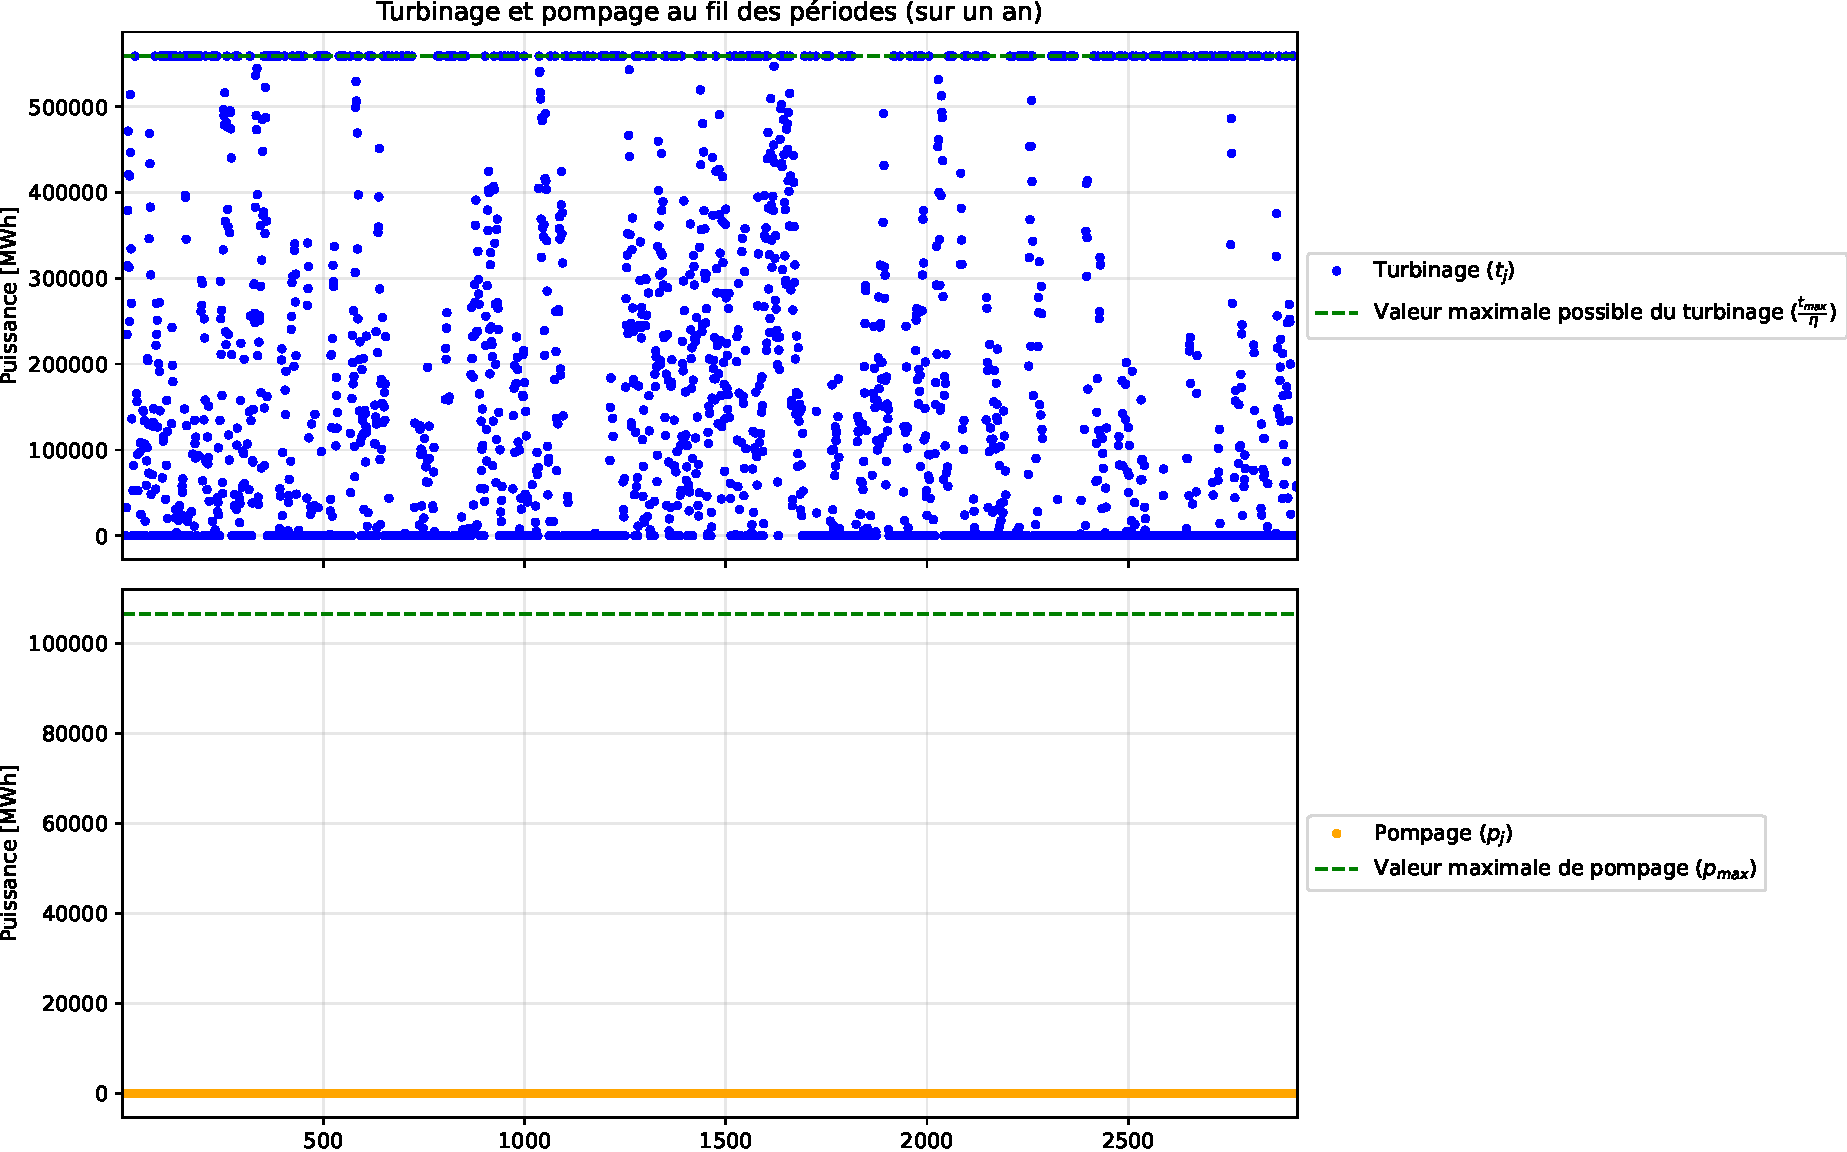
\includegraphics[scale=0.6]{GraphesP2/Turbinage_pompage_Q4.pdf}
    \caption{Représentation graphique du turbinage et du pompage
    influençant le niveau du bassin \eqref{eq:4A_contr2} pour le modèle de la question 4 par période de T = 3 heures sur un an.}
    \label{fig:Turbinage_pompage_Q4}
\end{figure}

\begin{figure}[h!]
    \centering
    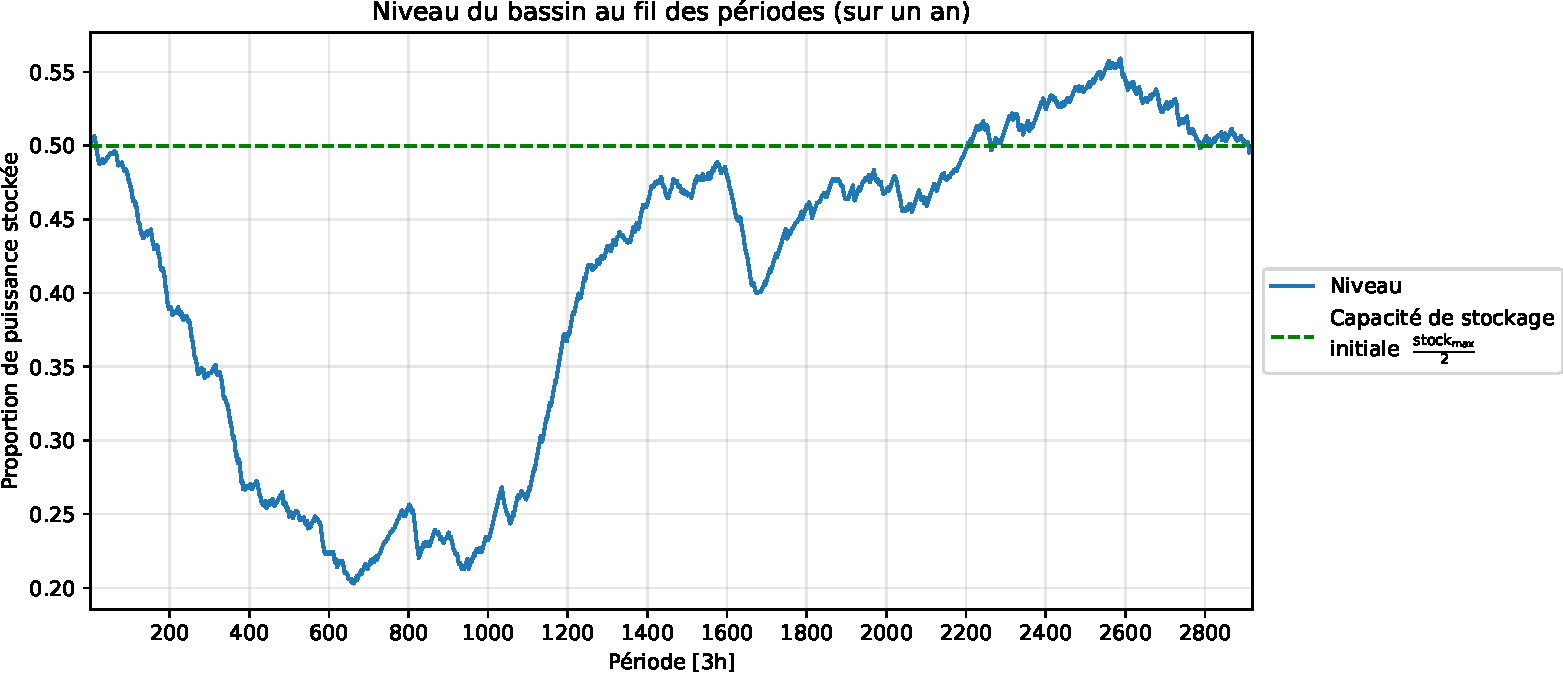
\includegraphics[scale=0.6]{GraphesP2/Niveau_Bassin_Q4.pdf}
    \caption{Représentation graphique du niveau du bassin \eqref{eq:4A_contr2} pour le modèle 
    de la question 4 par période de T = 3 heures sur un an.}
    \label{fig:Niveau_bassin_Q4}
\end{figure}

\begin{figure}[h!]
    \centering
    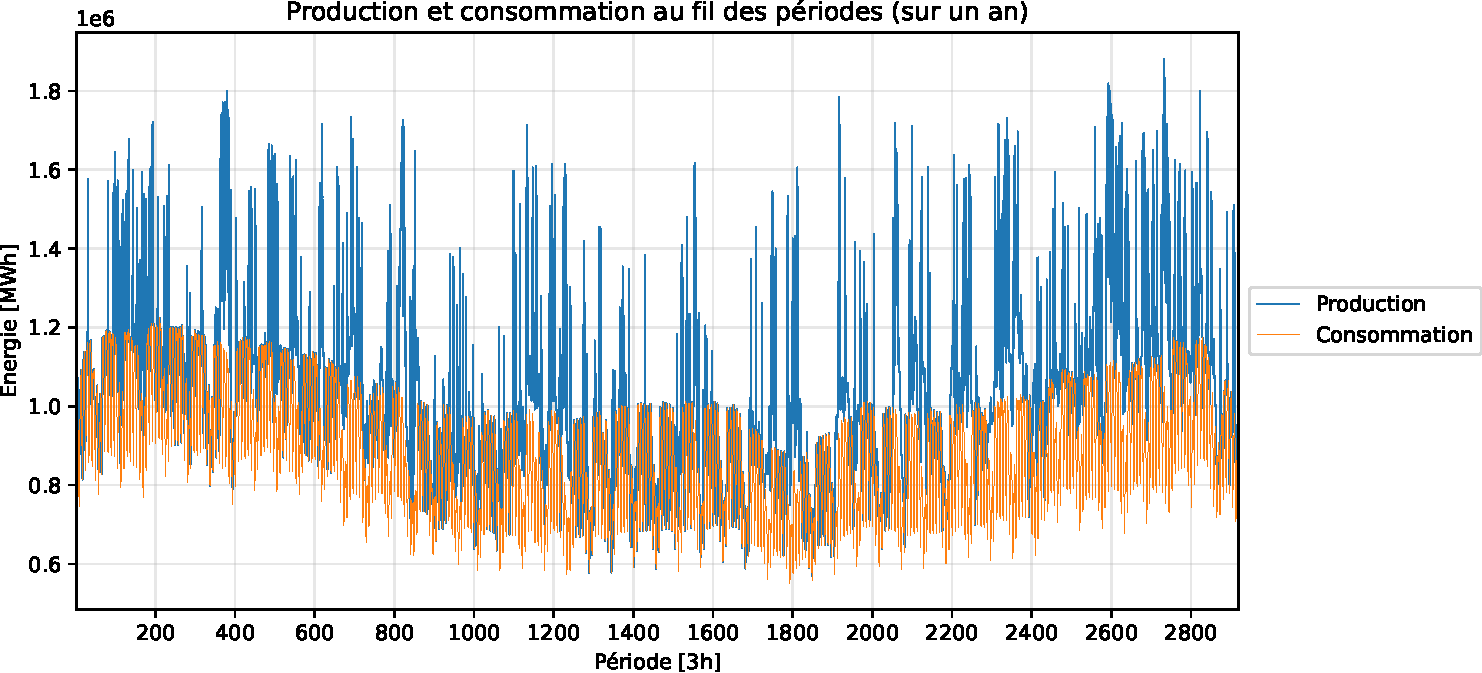
\includegraphics[scale=0.6]{GraphesP2/Prod_Cons_Q4.pdf}
    \caption{Représentation graphique de la production et de la consommation (en MWh) \eqref{eq:4A_contr1} pour le modèle de la question 4 
    par période de T = 3 heures sur un an.}
    \label{fig:Prod_Cons_Q4}
\end{figure}



\clearpage
\section*{Question 4C}
Pour traiter cette question, il faut s'intéresser au problème dual. Les résultats théoriques quant à l'influence des modifications des contraintes sur la fonction objectif s'obtiennent pour un problème sous forme standard.
En réajustant le modèle dans la bonne formulation, nous avons alors :
\begin{align}
    \min_{c_{i},t_j,p_j} \quad &\mathrm{costs}^\intercal\mathbf{c} \nonumber\\
    \textrm{tel que} \quad & \sum_{i=0}^{n-1} c_i e_i(j) + \eta \cdot t_j - p_j - s_{1,j} = \mathrm{cons}_j \quad \forall j \in  \{ 0, \ldots, m-1 \} \label{eq:4C_contr1}\\
    &\sum_{j=0}^{k} p_j - t_j + a_j + s_{2,k} =  \frac{\mathrm{stock}_\mathrm{max}}{2} \quad \forall k \in \{ 0, \ldots, m-2 \} \label{eq:4C_contr2}\\
    &\sum_{j=0}^{k} p_j - t_j + a_j - s_{3,k} =  -\frac{\mathrm{stock}_\mathrm{max}}{2} \quad \forall k \in \{ 0, \ldots, m-2 \} \label{eq:4C_contr3}\\
    & \sum_{j=0}^{m-1} p_j - t_j + a_j = 0\\
    &c_i + s_{4,j} = c_i^\mathrm{max} \quad \forall i \in  \{ 0, \ldots, n-1 \}\\
    &\eta \cdot t_j + s_{5,j} = t_\mathrm{max} \quad \forall j \in  \{ 0, \ldots, m-1 \} \label{eq:4C_contr6}\\
    &p_j + s_{6,j} = p_\mathrm{max} \quad \forall j \in  \{ 0, \ldots, m-1 \} \label{eq:4C_contr7}\\
    & c_i, t_j, p_j, s_{1,j}, s_{2,k}, s_{3,k}, s_{4,j}, s_{5,j}, s_{6,j} \geq 0
\end{align}
Où nous avons ajouté des variables d'écart $s_{\cdot,j}$ pour chaque contrainte contenant une inégalité.
Le problème dual s'écrit alors :
\begin{align*}
    \max_{y} \quad &b^\intercal y \quad\\ 
    \textrm{tel que} \quad &A^\intercal y \leq c\\
    & y \text{ libres}
\end{align*}
Les solutions de ce problème dual sont également données par le solver \verb|SCIPY| après la résolution du primal, ce qui nous permet de calculer les variations de la fonction objectif
lorsque nous modifions les capacités de stockage, de turbinage et de pompage.

\subsection*{Stockage}
Si nous augmentons d'une unité notre stockage, nous avons donc que $\mathrm{stock}_\mathrm{max} \leftarrow \mathrm{stock}_\mathrm{max} + 1$ (réassignation). Donc dans notre modèle,
notre vecteur $b$ est modifié, et devient $b$ plus un vecteur comprenant $\frac{1}{2}$ pour les contraintes 
\eqref{eq:4C_contr2}, $-\frac{1}{2}$ pour les contraintes \eqref{eq:4C_contr3} et 0 sinon. Si nous notons ce vecteur $\Delta b_{\mathrm{stock}}$, alors notre coût optimal augmentera de
$y^{* \intercal}\cdot \Delta b_{\mathrm{stock}}$ où $y^{*}$ est la solution du problème dual. Cela correspond en fait simplement à la somme des valeurs des variables duales associées aux contraintes
\eqref{eq:4C_contr2} et \eqref{eq:4C_contr3} multipliées par $\frac{1}{2}$ et $-\frac{1}{2}$ respectivement. Après l'implémentation en Python, nous avons que le coût optimal reste le même, donc \underline{l'augmentation de notre capacité de stockage d'une unité n'influence pas notre coût total}.

\subsection*{Pompage}
Nous pouvons procéder d'une manière similaire pour observer l'influence d'une augmentation de la capacité de pompage d'une valeur de $1 \unit{MW}$.
Puisque nous travaillons sur des périodes de $T = 3 \unit{h}$, la valeur de la contrainte \eqref{eq:4C_contr7} est modifiée de $p_\mathrm{max}$ à $p_\mathrm{max} + 3$. 
Nous sommons alors les valeurs des variables duales associées à cette contrainte que nous multiplions par $3$ pour obtenir la variation du coût optimal. 
Après l'implémentation en Python, nous avons que le coût optimal reste inchangé après l'augmentation de la capacité de pompage, donc \underline{l'augmentation de notre capacité de pompage d'une unité n'influence pas notre coût total}.

\subsection*{Turbinage}
Enfin, nous pouvons observer l'influence d'une augmentation de la capacité de turbinage d'une valeur de $1 \unit{MW}$.
Puisque nous travaillons sur des périodes de $T = 3 \unit{h}$, la valeur de la contrainte \eqref{eq:4C_contr6} est modifiée de $t_\mathrm{max}$ à $t_\mathrm{max} + 3$.
Nous sommons alors les valeurs des variables duales associées à cette contrainte que nous multiplions par $3$ pour obtenir la variation du coût optimal 
et nous obtenons que le coût optimal diminue d'une valeur de $\mathbf{1.583.760,79}$ \euro, soit environ $0.001$\% de diminution. Cette diminution peut être expliquée par le fait que nous pouvons profiter davantage de l'apport fluvial pour la consommation d'énergie et ainsi moins dépendre des installations éoliennes.\\ 

\noindent \textit{Tout notre raisonnement reste valide par rapport aux contraintes car nous considérons que pour des petites variations, notre solution reste admissible.}

\newpage
\section*{Question 5}
Nous devons à présent choisir, pour chaque site d'éoliennes, si nous installons $0\%, 50\%$ ou $100\%$ de la capacité maximale installable sur ce site.
Pour ce faire, nous rédéfinissons les variables $c_i$ de la question 4 :

\begin{table}[h!]
    \centering
    \renewcommand{\arraystretch}{1.5}% Add spacing between rows : default value is 1
    \begin{tabular}{|c || c |} 
        \hline
        Nom & Signification\\
        \hline\hline
        $c_{i} \in \{ 0, 1, 2 \}$ & Proportion de la capacité maximale $c_i^\mathrm{max}$ installée sur le i\textsuperscript{ème} site\\
        $t_j$ & Puissance à envoyer en turbinage choisie durant la j\textsuperscript{ème} période\\
        $p_j$ & Puissance de pompage choisie durant la j\textsuperscript{ème} période\\
        \hline
    \end{tabular}
    \caption{Table des nouvelles notations des variables de décisions utilisées pour le modèle de la question 5.}
    \label{table:notations_variables_5}
\end{table} 

\noindent La puissance installée sur le i\textsuperscript{ème} site équivaut alors à $0.5 \cdot c_ic_i^\mathrm{max}$. Le modèle devient alors :
\begin{align}
    \min_{c_{i} \in \mathbb{Z},t_j,p_j} \quad &\mathrm{costs}^\intercal 
    \begin{pmatrix}
        0.5 \cdot c_0c_0^\mathrm{max}\\
        \vdots\\
        0.5 \cdot c_{n-1}c_{n-1}^\mathrm{max}
    \end{pmatrix} \nonumber\\
    \textrm{tel que} \quad & \sum_{i=0}^{n-1} 0.5 \cdot c_ic_i^{max} e_i(j) + \eta \cdot t_j - p_j \ge \mathrm{cons}_j \quad \forall j \in  \{ 0, \ldots, m-1 \}\label{eq:5_contr1}\\
    & 0 \le \frac{\mathrm{stock}_\mathrm{max}}{2}  + \sum_{j=0}^{k} p_j - t_j + a_j \le  \mathrm{stock}_\mathrm{max} \quad \forall k \in \{ 0, \ldots, m-2 \}\label{eq:5_contr2}\\
    & \sum_{j=0}^{m-1} p_j - t_j + a_j = 0 \label{eq:5_contr3}\\
    & 0\le c_i \le 2 \quad \forall i \in  \{ 0, \ldots, n-1 \} \label{eq:5_contr4}  \\
    & 0 \le \eta \cdot t_j \le  t_\mathrm{max} \quad \forall j \in  \{ 0, \ldots, m-1 \} \label{eq:5_contr5}\\
    & 0 \le p_j \le  p_\mathrm{max} \quad \forall j \in  \{ 0, \ldots, m-1 \} \label{eq:5_contr6} 
\end{align}
Ici, seule les contraintes sur les $c_i$ ont été modifiées. Nous imposons maintenant que les $c_i$ soient des entiers compris entre 0 et 2 (compris).
La fonction objectif a également dû être adaptée selon notre nouveau choix de variables.\\ 
Pour la résolution de ce modèle, nous avons dû réduire la durée étudiée, en effet, nous avons tout d'abord
testé avec 2920 périodes (au complet), avec le solver par défaut de \verb|CVXPY|, nous avions dépassé les 180 minutes
d'exécution et avons alors arrêté. Nous avons ensuite testé avec le solver \verb|SCIPY| et avons arrêté au-dessus de 120
minutes. Nous avons en second lieu réduit le nombre de périodes à 1500, nous avions excédé les 65
minutes avec encore le solver \verb|SCIPY|. Enfin, nous avons défini le nombre de périodes à \textbf{1000}, et nous arrivons
à \textbf{46 minutes et 10.5 secondes} de calcul. Nous avons conclu que ce dernier choix de durée était raisonnable.
Ensuite, nous supposons que le coût d'installation des éoliennes
est réduit à la durée étudiée, c'est à dire que notre vrai vecteur de coûts sera donné par "$\frac{1000}{2920} \mathrm{costs}$".
Nous effectuons les calculs sur le solver pour le coût initial ($\mathrm{costs}$), ensuite nous ajustons 
par ce facteur ($\frac{1000}{2920}$) pour vous présenter les résultats.
\begin{table}[H]
    \centering
    \renewcommand{\arraystretch}{1.5}% Add spacing between rows : default value is 1
    \begin{tabular}{|c | c |} 
        \hline
        Modèle & Coût moyen (€/MWh) \\
        \hline
        Variables éoliennes discrètes (Question 5) & 44.914 \\
        \hline
        Variables éoliennes continues (Question 4) & 44.899 \\
        \hline
    \end{tabular}
    \caption{Comparaison des coûts moyens (ajustés par rapport à 1000 périodes) de la question 4 et 5.}
    \label{table:comparaison_resultat_Q5_Q4_1000}
\end{table} 
\noindent Nous constatons que le coût moyen a légèrement augmenté (bien que cela reste assez important à l'échelle
de l'Europe en termes de coût), c'est assez normal car nous restreignons les valeurs possibles d'installation 
de puissances de chaque site éolien, mais visiblement nous n'avons pas une augmentation si importante, peut-être par le fait 
que lors de la résolution de la question 4 (\autoref{fig:Capacité_Eolienne_Q4}), nous n'avions pas tellement de sites
comportant des valeurs de capacités installées intermédiaires, mais plus concentrées à 0 et à 1. Nous illustrons la différence sur le choix de l'installation 
de la capacité éolienne en fonction de notre modèle avec des variables discrètes et continues. Nous pouvons voir que le turbinage est un peu plus varié qu'à la question 4, moins de valeurs extrêmes (au maximum/minimum), et cette fois-ci,
le pompage est exploité contrairement à la question 4 où il est nul sur toute la période étudiée. 
Nous remontons encore une fois bien au niveau initial à la fin de la période.  
Nous constatons que la production est beaucoup plus proche de la consommation par rapport à la question précédente.
\begin{figure}[h!]
    \centering
    \includegraphics[scale=0.6]{GraphesP2/Capacité_Eolienne_Q5.pdf}
    \caption{Représentation graphique de la proportion de la capacité éolienne installée sur chaque site pour le modèle de la question 5 en comparaison
    avec le modèle de la question 5, par période
    de T = 3 heures sur 1000 périodes.}
    \label{fig:Capacité_Eolienne_Q5}
\end{figure}

\begin{figure}[H]
    \centering
    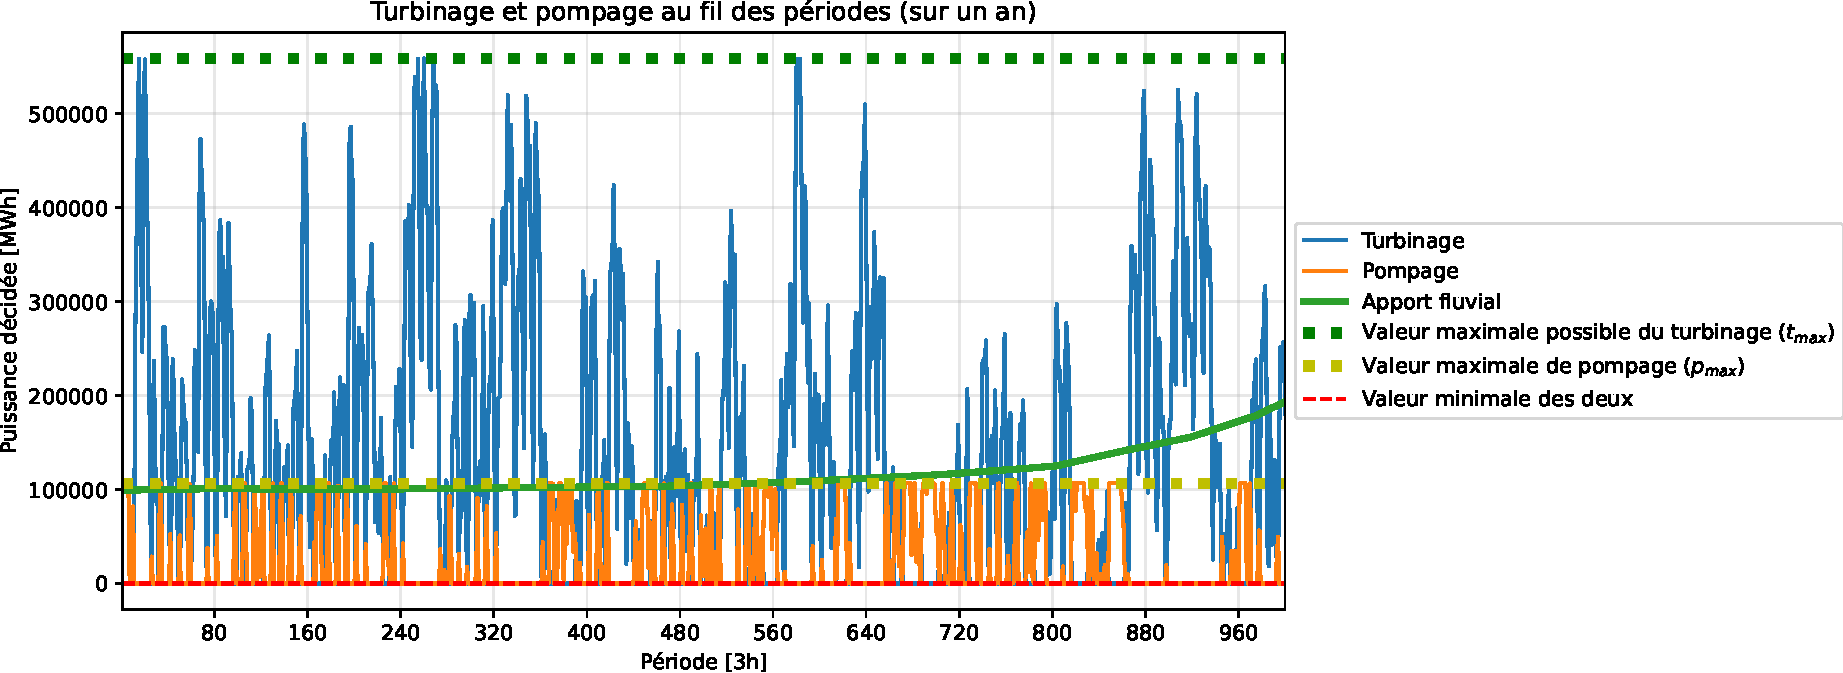
\includegraphics[scale=0.6]{GraphesP2/Turbinage_pompage_Q5.pdf}
    \caption{Représentation graphique du turbinage et du pompage
    influençant le niveau du bassin \eqref{eq:5_contr2} pour le modèle de la question 4 par période de T = 3 heures sur 1000 périodes.}
    \label{fig:Turbinage_pompage_Q5}
\end{figure}

\begin{figure}[H]
    \centering
    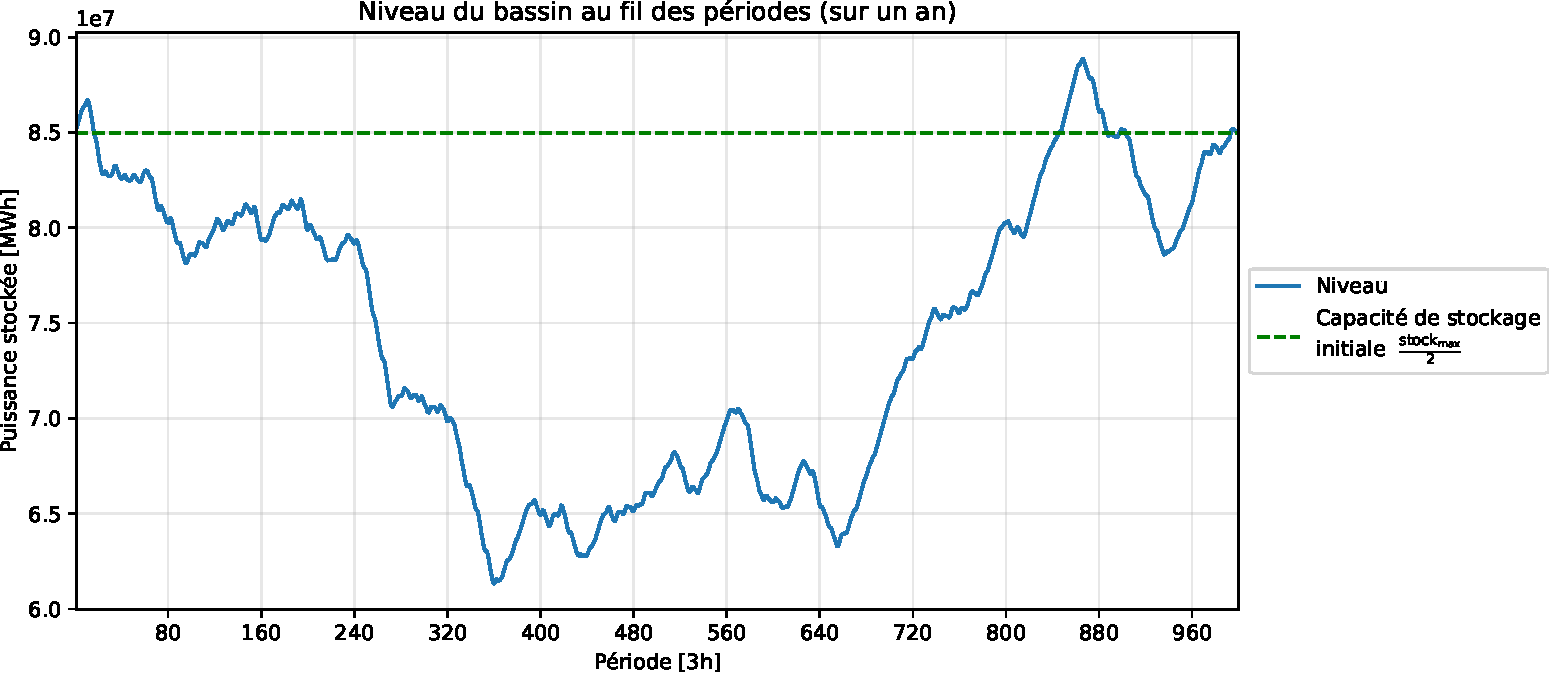
\includegraphics[scale=0.6]{GraphesP2/Niveau_Bassin_Q5.pdf}
    \caption{Représentation graphique du niveau du bassin \eqref{eq:5_contr2} pour le modèle 
    de la question 5 par période de T = 3 heures sur 1000 périodes.}
    \label{fig:Niveau_bassin_Q5}
\end{figure}

\begin{figure}[H]
    \centering
    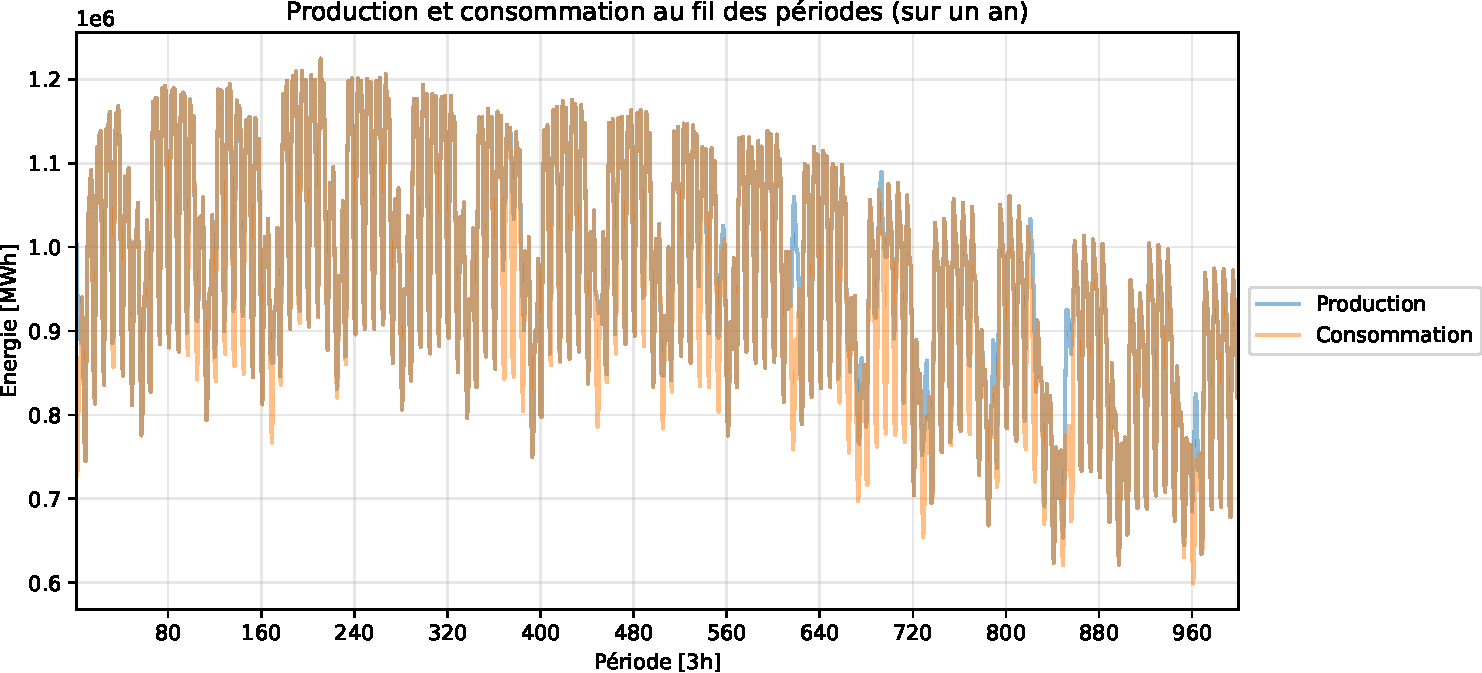
\includegraphics[scale=0.6]{GraphesP2/Prod_Cons_Q5.pdf}
    \caption{Représentation graphique de la production et de la consommation (en MWh) 
    \eqref{eq:5_contr1} pour le modèle de la question 5 par période de T = 3 heures sur 1000 périodes.}
    \label{fig:Prod_Cons_Q5}
\end{figure}

\clearpage

\section*{Question 6}
Pour ce dernier modèle, nous avons également la possibilité d'installer des centrales à gaz, qui peuvent être utilisées pour produire de l'électricité en cas de besoin.
La puissance totale à installer fait partie des variables de décision, ainsi que l'énergie produite par ces centrales en chaque période de $T \unit{h}$.\\
Nous avons donc les nouvelles variables suivantes :

\begin{table}[h!]
    \centering
    \renewcommand{\arraystretch}{1.5}% Add spacing between rows : default value is 1
    \begin{tabular}{|c || c |} 
        \hline
        Nom & Signification\\
        \hline\hline
        $c_i$ & Capacité éolienne installée sur le i\textsuperscript{ème} site\\
        $t_j$ & Puissance à envoyer en turbinage choisie durant la j\textsuperscript{ème} période\\
        $p_j$ & Puissance de pompage choisie durant la j\textsuperscript{ème} période\\
        $g_\mathrm{tot}$ & Puissance totale à installer pour les centrales à gaz\\
        $g_j$ & \'Energie produite par les centrales à gaz durant la j\textsuperscript{ème} période\\
        \hline
    \end{tabular}
    \caption{Table des notations des variables de décisions utilisées pour le modèle de la question 6.} 
    \label{table:notations_variables_6}
\end{table}

\noindent Nous devons alors prendre en compte, en plus du coût d'installation des éoliennes, le coût d'installation des centrales à gaz ainsi que leur coût de fonctionnement.
Le modèle devient alors :

\begin{align}
    \min_{c_{i},t_j,p_j} \quad &\mathrm{costs}^\intercal\mathbf{c} + \mathrm{gas\_prod\_cost}\cdot \sum_{j=0}^{m-1} g_j + \mathrm{gas\_install\_cost} \cdot g_\mathrm{tot}\nonumber\\
    \textrm{tel que} \quad & \sum_{i=0}^{n-1} c_i e_i(j) + g_j + \eta \cdot t_j - p_j \ge \mathrm{cons}_j \quad \forall j \in  \{ 0, \ldots, m-1 \}\label{eq:6_contr1}\\
    & 0 \le \frac{\mathrm{stock}_\mathrm{max}}{2}  + \sum_{j=0}^{k} p_j - t_j + a_j \le  \mathrm{stock}_\mathrm{max} \quad \forall k \in \{ 0, \ldots, m-2 \}\label{eq:6_contr2}\\
    & \sum_{j=0}^{m-1} p_j - t_j + a_j = 0 \label{eq:6_contr3}\\
    & 0 \le c_i \le c_i^\mathrm{max} \quad \forall i \in  \{ 0, \ldots, n-1 \}  \label{eq:6_contr4}\\
    & 0 \le \eta \cdot t_j \le  t_\mathrm{max} \quad \forall j \in  \{ 0, \ldots, m-1 \}  \label{eq:6_contr5}\\
    & 0 \le p_j \le  p_\mathrm{max} \quad \forall j \in  \{ 0, \ldots, m-1 \} \label{eq:6_contr6}\\
    & 0 \le g_j \le g_\mathrm{tot} \quad \forall j \in  \{ 0, \ldots, m-1 \} \label{eq:6_contr7}
\end{align}

\noindent où $\mathrm{gas\_prod\_cost}$ est le coût de production d'énergie par les centrales à gaz et $\mathrm{gas\_install\_cost}$ est le coût d'installation des centrales à gaz.\\
La fonction objectif tient maintenant compte du coût d'installation et de production des centrales à gaz. La contrainte \eqref{eq:6_contr1} est modifiée pour prendre en compte la production d'énergie par les centrales à gaz dans le bilan total de production. 
Enfin, une dernière contrainte \eqref{eq:6_contr7} est ajoutée pour limiter la production d'énergie par les centrales à gaz à la puissance totale installée.
Après la résolution numérique, nous obtenons une valeur moyenne de $\mathbf{48.15}$ \euro/MWh, ce qui est mieux que 
le résultat de la question 4 ($\mathbf{58.282}$ \euro/MWh). Cela peut s'expliquer par le fait que nous
avons plus de possibilités, dans le sens que nous pouvons ajuster la production avec un levier en plus,
ce qui fait que nous pouvons mieux répartir notre production énergétique afin de minimiser le coût. \\
L'introduction des variables concernant le gaz ne semblent pas avoir influencé les capacités éoliennes installées 
par rapport à la question 4 (\autoref{fig:Capacité_Eolienne_Q4} / \autoref{fig:Q60}). 
Le pompage est cette fois plus utilisé que dans la question 4 (\autoref{fig:Turbinage_pompage_Q4})
Bien que délicat à bien illustrer, nous pouvons voir que les valeurs de production et de consommation sont 
assez proches.

\begin{figure}[h!]
    \centering
    \includegraphics[scale=0.6]{GraphesP2/Capacité_Eolienne_Q6.pdf}
    \caption{Représentation graphique de la proportion de la capacité éolienne installée sur chaque site pour le modèle de la question 6 par période
    de T = 3 heures sur une année.}
    \label{fig:Q60}
\end{figure}

\begin{figure}[H]
    \centering
    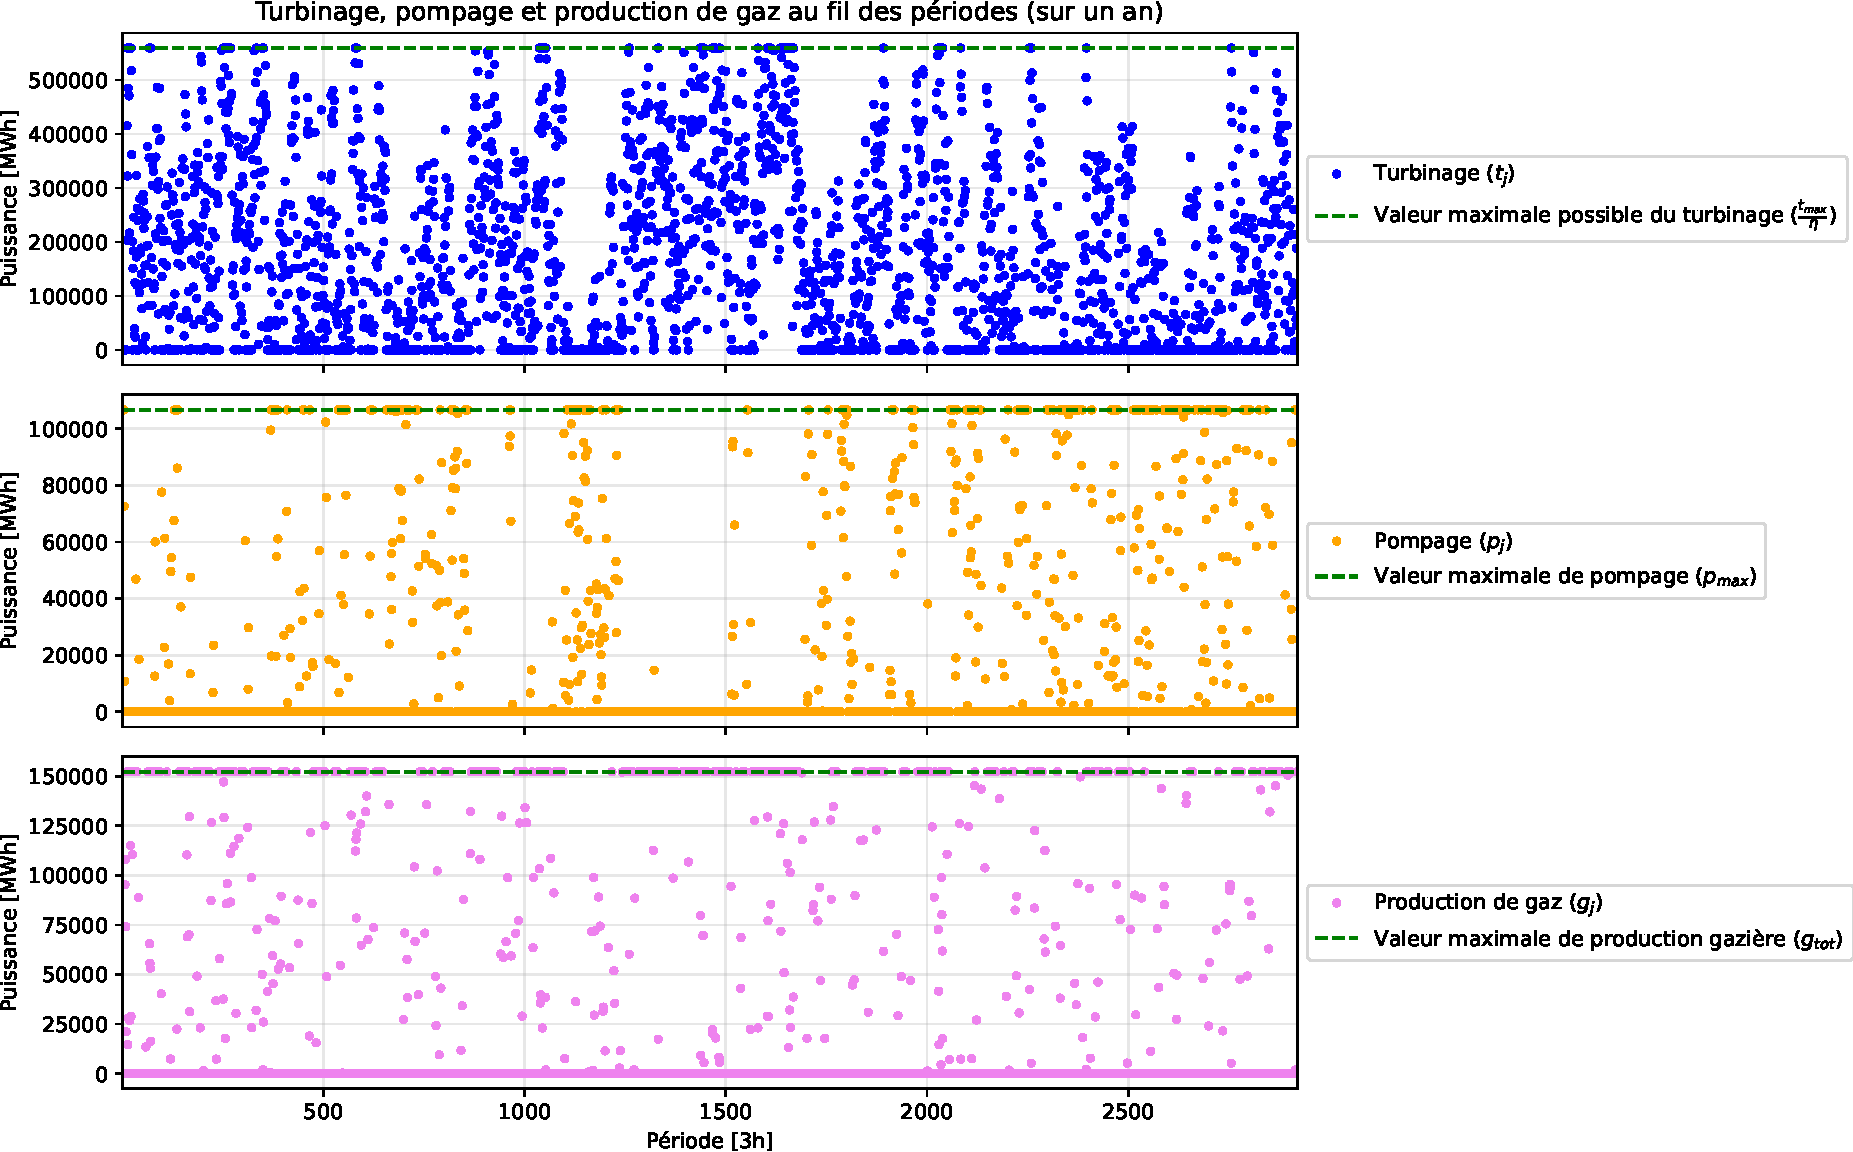
\includegraphics[scale=0.6]{GraphesP2/Productions_Q6.pdf}
    \caption{Représentation graphique du turbinage et du pompage
    influençant le niveau du bassin \eqref{eq:6_contr2} ainsi que de la production de gaz pour le modèle de la question 6 par période de T = 3 heures sur un an.} 
    \label{fig:Q61}
\end{figure}

\begin{figure}[h!]
    \centering
    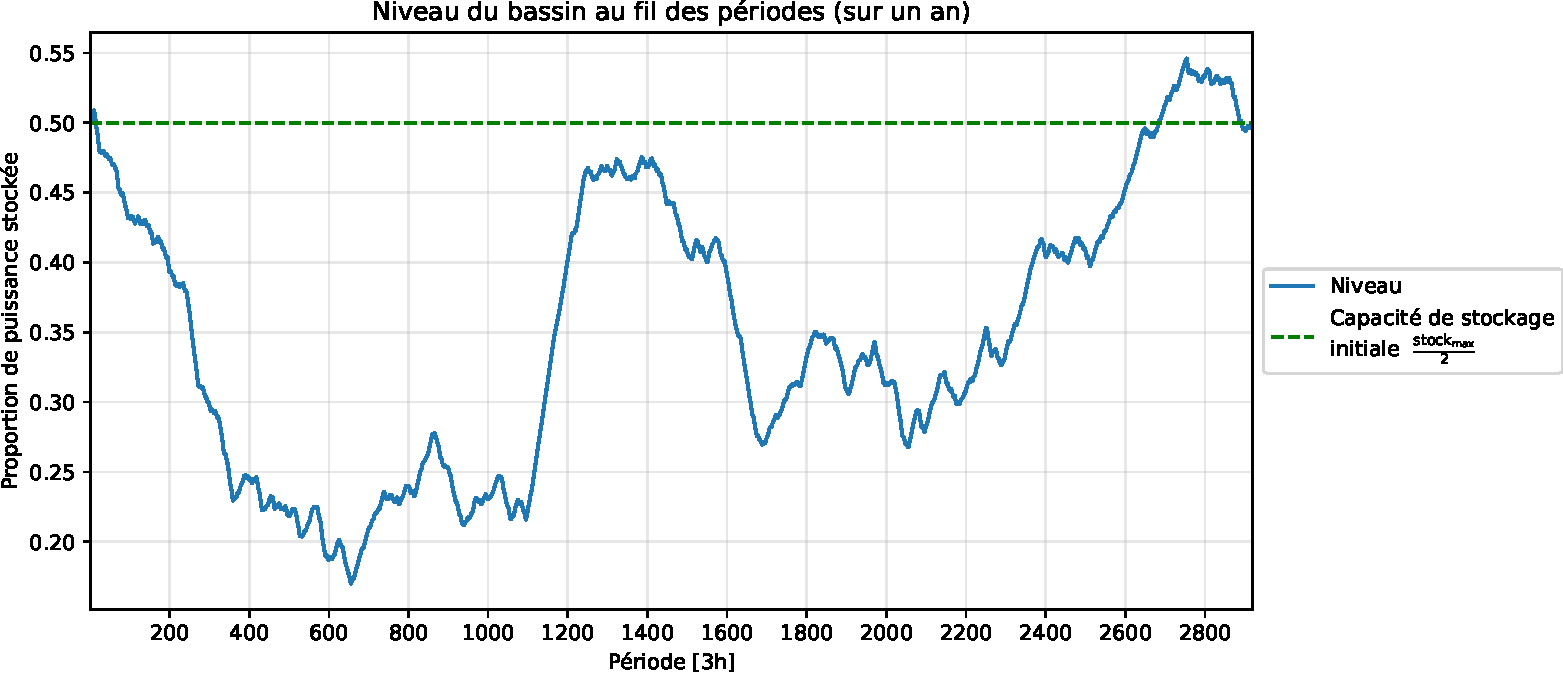
\includegraphics[scale=0.6]{GraphesP2/Niveau_Bassin_Q6.pdf}
    \caption{Représentation graphique du niveau du bassin \eqref{eq:6_contr2} pour le modèle 
    de la question 6 par période de T = 3 heures sur 1000 périodes.} 
    \label{fig:Q62}
\end{figure}

\begin{figure}[H]
    \centering
    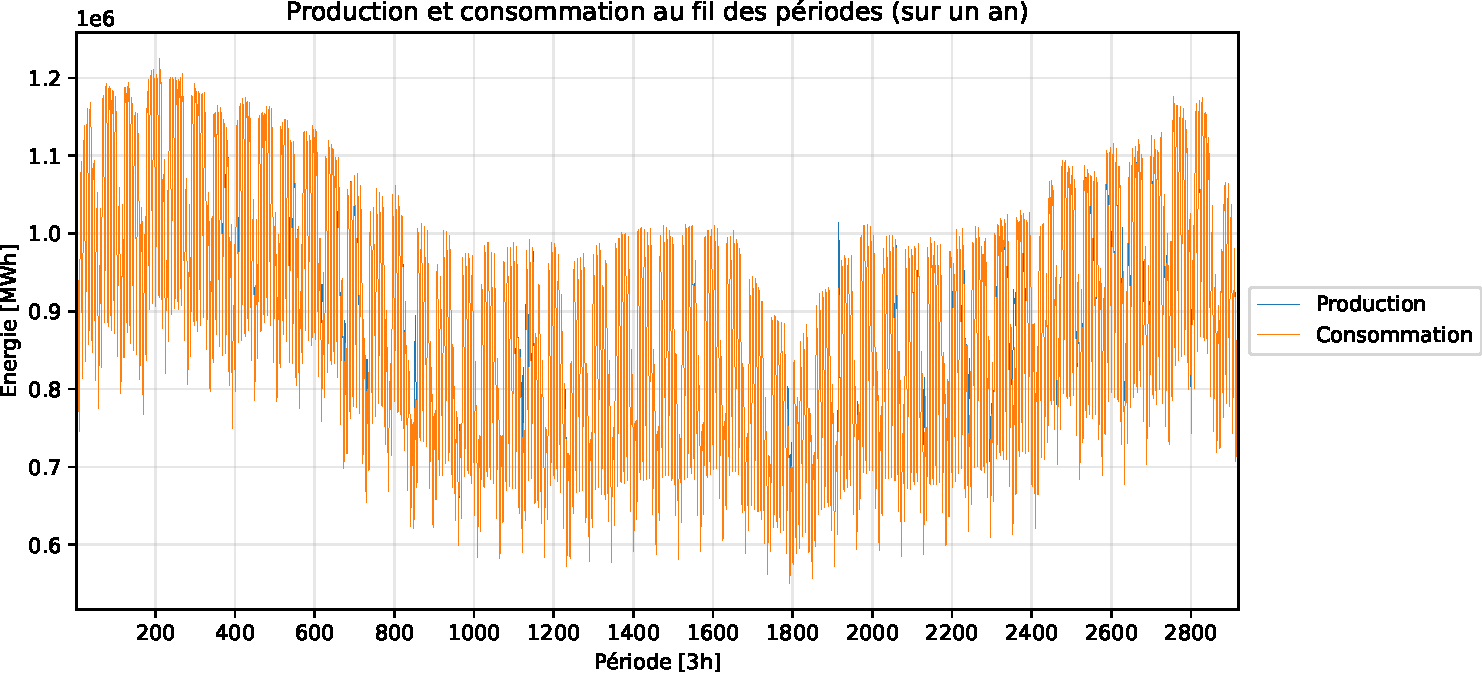
\includegraphics[scale=0.6]{GraphesP2/Prod_Cons_Q6.pdf}
    \caption{Représentation graphique de la production et de la consommation (en MWh) 
    \eqref{eq:6_contr1} pour le modèle de la question 6 par période de T = 3 heures sur un an.} 
    \label{fig:Q63}
\end{figure}

\end{document}
